
%\newcommand{\MLP}{\text{MLP}}
%\newcommand{\FeedForward}{\text{FeedForward}}
%\newcommand{\Softmax}{\text{Softmax}}
%\newcommand{\reals}{\mathbb{R}}
\def\m{m}


\section{The Abstractor Framework}
\label{sec:abstractor_framework}

At a high level, the primary function of an Abstractor is to compute abstract relational features of its
inputs.\footnote{In this paper, we will tend to use the name `Abstractor' to refer to both the module, the framework, and models which contain the Abstractor module as a main component.} That is, given a set or sequence of input objects $o_1, \ldots, o_\m$, the relational Abstractor learns to model a relation $r(\cdot, \cdot)$ and computes a function on
the set of pairwise relations between objects ${\{ r(o_i, o_j) \}}_{ij}$. The relations and the computations on them are learned to carry out a specific prediction task. This learning is often end-to-end, but, crucially, the Abstractor framework naturally supports modular learning.
\subsection{Relational symbolic message-passing}
\label{ssec:message_passing}

At the core of Abstractors is an operation we refer to as \textit{relational symbolic message-passing}.
The input to this operation is a relation tensor $R = \left[r(o_i, o_j)\right]_{i,j=1}^\m$, where $r(o_i, o_j) \in \mathbb{R}^{d_r}$ is a vector describing the relation between object $o_i$ and object $o_j$. We will come back to how an Abstractor models pairwise relations and computes the relation tensor in the next subsection.

The starting point of symbolic message-passing is a set of learnable symbols $s_1, \ldots, s_\m \in \mathbb{R}^{d_s}$, where the hyperparameter $d_s$ is the dimension of the symbolic vectors. We call these parameters \textit{symbols} because each of them references (or ``is bound to'') a particular object, but they are independent of the values of these objects. That is, the $i$th symbol references the $i$th object, but the value of $s_i$ is independent of the value of $o_i$. The use of these learned, input-independent symbols is how symbolic message-passing achieves its abstraction.

In relational symbolic message-passing, we perform message-passing on these learned symbolic parameters according to the relation tensor $R$. In general, this message-passing operation can be described as a set-valued function of the form
\begin{equation}
    \label{eq:symbolic_message_passing}
    s_i \leftarrow \text{Update}\Big( s_i, \ \left\{ \left(R[i,j], s_j\right)\right\}_{j\in[m]}\Big), \quad i = 1, \ldots, m.
\end{equation}

That is, the value of the $i$th symbol is updated as a function of the set of tuples $(R[i,j], s_j)$ of the relations with all other objects and the symbols of these objects. The symbols $s_j$ are naturally viewed as values on the nodes of a graph, and the relations $R[i,j]$ are naturally viewed as weights on the edges. A simple but important special case of this is linear message-passing
\begin{equation}
    \label{eq:linear_symbolic_mp}
    s_i \leftarrow \sum_{j=1}^{m} R[i,j] s_j, \quad i=1, \ldots, m
\end{equation}

In the above, if $d_r > 1$, the operation should be read as
\begin{equation*}
    R[i,j] s_j = \left( R[i,j,1] s_j, \ldots, R[i,j, d_r] s_j \right) \in \reals^{d_s \times d_r},
\end{equation*}

where $d_r$ is the dimension of the relation. That is, the result is concatenated.

Following message-passing, each updated symbol $s_i$ can be passed through a feedforward neural network $\phi: \reals^{d_s \times d_r} \rightarrow \reals^{d_a}$ to compute a non-linear function of the output. This also controls the dimension of the symbols so that it doesn't grow by a factor of $H$ with each layer (e.g., take $d_a = d_s$). Empirically, a residual connection and layer normalization may be useful.

This message-passing operation can be repeated multiple times to iteratively update the symbolic vectors.  The output of relational symbolic message-passing is the set of symbols $\bm{A}$ at the end of this sequence of message-passing operations. This is summarized in~\Cref{alg:symbolic_mp}.

\begin{algorithm}[ht!]
	\caption{Symbolic Message-Passing}\label{alg:symbolic_mp}
	\SetKwInOut{Input}{Input}
	\SetKwInOut{Output}{Output}
	\SetKwInOut{LearnableParams}{Learnable parameters{\ }}
	\SetKwInOut{HyperParams}{Hyperparameters}

	\Input{Relation tensor: \(R \in \mathbb{R}^{\m \times \m \times d_r}\)}
	\HyperParams{\(L,\ d_s, d_a\), hyperparameters of feedforward networks}
	\LearnableParams{symbols \(\bm{S} = (s_1, \ldots, s_\m) \in \reals^{d_s \times \m}\), feedforward networks \(\phi^{(1)}, \ldots, \phi^{(L)}\)}
	\Output{Abstracted sequence: \(\bm{A} = (a_1, \ldots, a _\m) \in \reals^{d_a \times \m}\)}
	\vspace{1em}

	\((a_1, \ldots, a_\m) \gets (s_1, \ldots, s_\m)\)

	\For{\(l \gets 1\) \KwTo \(L\)}{
		\(a_i \gets \sum_{j=1}^{n} R[i,j] a_j, \quad i = 1, \ldots, \m\)

		\(a_i \gets \phi^{(l)}(a_i), \quad i = 1, \ldots, \m\)
	}
\end{algorithm}


\subsection{Multi-head relations and relational cross-attention}

Next, we turn our attention to how the Abstractor models pairwise relations and computes the relation tensor $R \in \mathbb{R}^{\m \times \m \times d_r}$.

The inner product operation is a natural way to capture notions of relations and similarity. In Euclidean space, inner products capture the geometric alignment between vectors. Similarly, for arbitrary objects with vector representations, inner products between these vector representations can capture relations between these objects.

We model pairwise relations as inner products between appropriately encoded (or `filtered') object representations. In particular, we model the pairwise relation function $r(\cdot, \cdot) \in \mathbb{R}^{d_r}$ in terms $d_r$ learnable `left encoders' $\phi_1, \ldots, \phi_{d_r}$, and $d_r$ `right encoders' $\psi_1, \ldots, \psi_{d_r}$,
% \begin{equation}\label{eq:multi_head_rel}
%     r(x,y) = \left(\langle \phi_1(x), \psi_1(y) \rangle, \langle \phi_2(x), \psi_2(y) \rangle, \ldots, \langle \phi_{d_r}(x), \psi_{d_r}(y) \rangle \right)^\top \in \mathbb{R}^{d_r}.
% \end{equation}

\begin{equation}\label{eq:multi_head_rel}
    r(x,y) = \begin{pmatrix}\langle \phi_1(x), \psi_1(y) \rangle \\ \vdots \\ \langle \phi_{d_r}(x), \psi_{d_r}(y) \rangle \end{pmatrix} \in \mathbb{R}^{d_r}.
\end{equation}


In general, $\phi_i, \psi_j$ can be any learnable maps. These transformations can be thought of as \textit{relational filters}. They extract a particular attribute of the objects such that an inner product of the transformed objects indicates the alignment or similarity along this attribute. Having several different filters allows for modeling rich multi-dimensional relations. This is one notable advantage of this formulation over the CoRelNet model \citep{kerg2022neural}, which processes a \textit{1-dimensional} similarity matrix as input to a multi-layer perceptron. In the next section, we analyze the class of functions that the multi-head relation module can model.

In order to promote weight sharing, we focus our attention to inner product relations of the form

\begin{equation}\label{eq:inner_prod_rel_weight_sharing}
    r(x,y) = \begin{pmatrix} \left\langle W_1^{(1)}\phi(x), W_2^{(1)} \phi(y) \right\rangle \\  \vdots \\ \left\langle W_1^{(d_r)}\phi(x), W_2^{(d_r)} \phi(y) \right\rangle \end{pmatrix} \in \mathbb{R}^{d_r},
\end{equation}

\noindent where $\phi$ is a common non-linear map, and $W_1^{(i)}, W_2^{(i)}$ are projection matrices for each dimension of the relation. For general functions $\phi$, this class of functions is no smaller than the one above (e.g., take $\phi$ to be the concatenation of $\phi_1, \ldots, \phi_{d_r}, \psi_1, \ldots, \psi_{d_r}$ and $W_1^{(i)}, W_2^{(i)}$ to be the projection matrices which extract the appropriate components), but does enable greater weight sharing.

We refer to this operation as \textit{Multi-Head Relation} (\Cref{alg:multiheadrelation}). In our implementation, computation of the inner product is done efficiently with Einstein summation. Also, we add a hyperparameter to control whether the relations are modeled as symmetric or asymmetric (as in the description above). If the relations are to be modeled as symmetric, we set $W_1^{(i)} = W_2^{(i)}$. For certain tasks where relations may be naturally symmetric, this may be a useful inductive bias which improves sample-efficiency (e.g., see the discussion in~\cite{kerg2022neural}).

\begin{algorithm}[ht!]
	\caption{Multi-Head Relation (MHR) module}\label{alg:multiheadrelation}
	\SetKwInOut{Input}{Input}
	\SetKwInOut{Output}{Output}
	\SetKwInOut{LearnableParams}{Learnable parameters{\ }}
	\SetKwInOut{HyperParams}{Hyperparameters}

	\Input{sequence of objects: $\bm{X} = (x_1, \ldots, x_\m) \in \reals^{d}$ }
	\HyperParams{Dimension of relation $d_r$, Projection dimension $d_p$, dimension of embedding $d_e$}
	\LearnableParams{projection matrices $W_1^{(i)}, W_2^{(i)} \in \reals^{d_p \times d_e}, \ i=1, \ldots, d_r$, embedder network $\phi: \reals^d \to \reals^{d_e}$}
	\Output{Relation tensor $R \in \reals^{\m \times \m \times d_r}$}
	\vspace{1em}

	\For{\(i,j \gets 1\) \KwTo \(\m\)}{
        \For{$k \gets 1 $ \KwTo $d_r$}{
            $R[i, j, k] \gets \langle W_1^{(k)} \phi(x_i), W_2^{(k)} \phi(x_j)\rangle$
        }
	}
\end{algorithm}

\subsection{The Abstractor module: Putting it all together}

The above two sections provide a complete description of relational symbolic message-passing and computing relations via multi-head relation modules. These are the two main components of the Abstractor module.

The initial abstract state is $\bm{S} = (s_1, \ldots, s_\m)$ with abstract symbols $s_j$ that are task-dependent but input-independent, trainable using backpropagation. The multi-head relation module learns relations among the input objects and uses those relations to transform the abstract state. Importantly, each `head' of the multi-head relation module encode learned relations and attributes which can be reused across tasks.

Only relational information, computed through inner products, is used to transform the abstract variables; no information about the individual object representations themselves is directly accessed by the abstract side. This enables greater out-of-distribution generalization ability since it allows for the representations of the objects to change as long as the transformed inner products are approximately preserved (see~\Cref{sec:experiments} for experiments exploring this). This is a crucial component of the idea of the relational bottleneck.

\Cref{alg:abstractor} provides an algorithmic description of the archetypical Abstractor.

\begin{algorithm}[ht!]
	\caption{Abstractor}\label{alg:abstractor}
	\SetKwInOut{Input}{Input}
	\SetKwInOut{Output}{Output}
	\SetKwInOut{LearnableParams}{Learnable parameters}
	\SetKwInOut{HyperParams}{Hyperparameters}

	\Input{sequence of objects: $\bm{X} = (x_1, \ldots, x_\m) \in \reals^{d}$ }
	\HyperParams{\# of layers \(L\), dim of symbols \(d_s\), dim of abstract objects \(d_a\), hyperparameters of MHR modules, activation function for relation tensor \(\sigma_{\mathrm{rel}}\), hyperparameters of feedforward networks.}
	\LearnableParams{symbols \(\bm{S} = (s_1, \ldots, s_\m) \in \reals^{d_s \times \m}\), feedforward networks \(\phi^{(1)}, \ldots, \phi^{(L)}\), parameters of MHR modules.}
	\Output{Abstracted sequence: \(\bm{A} = (a_1, \ldots, a _\m) \in \reals^{d_a \times \m}\)}
	\vspace{1em}

	\((a_1, \ldots, a_\m) \gets (s_1, \ldots, s_\m)\)

	\For{\(l \gets 1\) \KwTo \(L\)}{
        \(R \gets \text{MultiHeadRelation}^{(l)}(\bm{X}) \)

        \(R \gets \sigma_{\mathrm{rel}}(R)\)

		\(a_i \gets \sum_{j=1}^{n} R[i,j] a_j, \quad i = 1, \ldots, \m\)

		\(a_i \gets \phi^{(l)}(a_i), \quad i = 1, \ldots, \m\)
	}
\end{algorithm}

Note that the relation tensor output by the multi-head relation module is processed with an activation function $\sigma_{\mathrm{rel}}$. Depending on the task, one good choice for this is the softmax activation function. This normalizes the message-passing operation such that each abstract symbol is updated as a \textit{convex combination} of the other symbols based on the relation tensor. It is important to note that this causes the computed relation between two objects to depend also on the relations with other objects (i.e., $R[i,j]$ depends not only on $x_i, x_j$, but on the full object sequence). Thus, softmax computes the relation between two objects \textit{relative} to the relations with all objects. Depending on the application, this may be a very useful inductive bias or a harmful one. Alternatively, we may apply an activation function $\sigma_{\mathrm{rel}}$ independently for each entry in the relation tensor (e.g., linear, relu, sigmoid, tanh, etc.)

Finally, we remark that this operation is closely related to the multi-head attention operation of Transformers. In fact, computing the relation tensor and performing symbolic message-passing can be achieved via a multi-head attention operation of the form
\begin{equation}\label{eq:relation_crossattention}
    \text{RelationalCrossAttention}\left(E, S\right) \equiv \text{Attention}\left( Q \gets E, K \gets E, V \gets S \right),
\end{equation}
where $E$ are the input objects (or some processed-encoding of them), and $S = (s_1, \ldots, s_\m)$ are the symbolic variables. We refer to this operation as \textit{relational cross-attention}. This is in contrast to standard (encoder-decoder) cross-attention, which takes the form $\text{Attention}\left( Q \gets D, K \gets E, V \gets E \right)$.

For completeness, ~\Cref{alg:relational_abstractor} gives an algorithmic description of the Abstractor module, cast in terms of Transformer-based attention mechanisms. Note that we have added a self-attention operation performed on the abstract symbols. This is merely to show this as an option. It may be useful for some tasks, but, unlike the rest of Abstractor, it not intuitive what this might be computing.

\begin{algorithm}[th!]
    \caption{Abstractor (cast in terms of Transformer operations)}\label{alg:relational_abstractor}
    \SetKwFor{For}{for}{do}{end}
    \SetKwInOut{Input}{Input}
    \SetKwInOut{Output}{Output}
    \SetKwInOut{LearnableParams}{Learnable parameters{\ }}
    \SetKwInOut{HyperParams}{Hyperparameters}

    \Input{sequence of objects: $\bm{X} = (x_1, \ldots, x_\m) \in \reals^{d}$ }
	\HyperParams{\# of layers \(L\), dim of symbols \(d_s\), dim of abstract objects \(d_a\), hyperparameters of attention modules, hyperparameters of feedforward networks.}
	\LearnableParams{symbols \(\bm{S} = (s_1, \ldots, s_\m) \in \reals^{d_s \times \m}\), feedforward networks \(\phi^{(1)}, \ldots, \phi^{(L)}\), parameters of attention modules.}
	\Output{Abstracted sequence: \(\bm{A} = (a_1, \ldots, a _\m) \in \reals^{d_a \times \m}\)}

    \vspace{1em}

    $\bm{A} \gets \bm{S}$

    \For{$l \gets 1$ \KwTo $L$}{
        $\bm{A} \gets \text{SelfAttention}^{(l)}(\bm{A})$\;
        $\bm{A} \gets \text{RelationalAttention}^{(l)}(\bm{X}, \bm{S})$\;
        $\bm{A} \gets \phi^{(l)}(\bm{A})$\;
        }
\end{algorithm}

\subsection{Relational learning using Transformers}

The Abstractor module fits naturally into Transformer models. Hence, we position the Abstractor framework as an extension of Transformers. In particular, combining an Abstractor with Transformer Encoder and Decoder modules forms a powerful sequence model with enhanced abilities for relational reasoning and abstraction.

In our extended framework, processing occurs in encoder/decoder modules that handle particular types of information,
separated from modules for ``abstract inference.'' The encoders/decoders and the Abstractor modules communicate
through cross-attention mechanisms that couple abstract states with specific information in encoder/decoder modules.  The abstract layers are composable to include a hierarchy of abstract modules in which higher order relations are learned from lower level relations, analogous to how convolutional layers are composed in deep neural networks.

%\begin{figure}[t]
    \begin{wrapfigure}{R}{0.50\textwidth}
        \vspace{-3mm}
        \begin{center}
        \begin{tabular}{c}
            \hskip5pt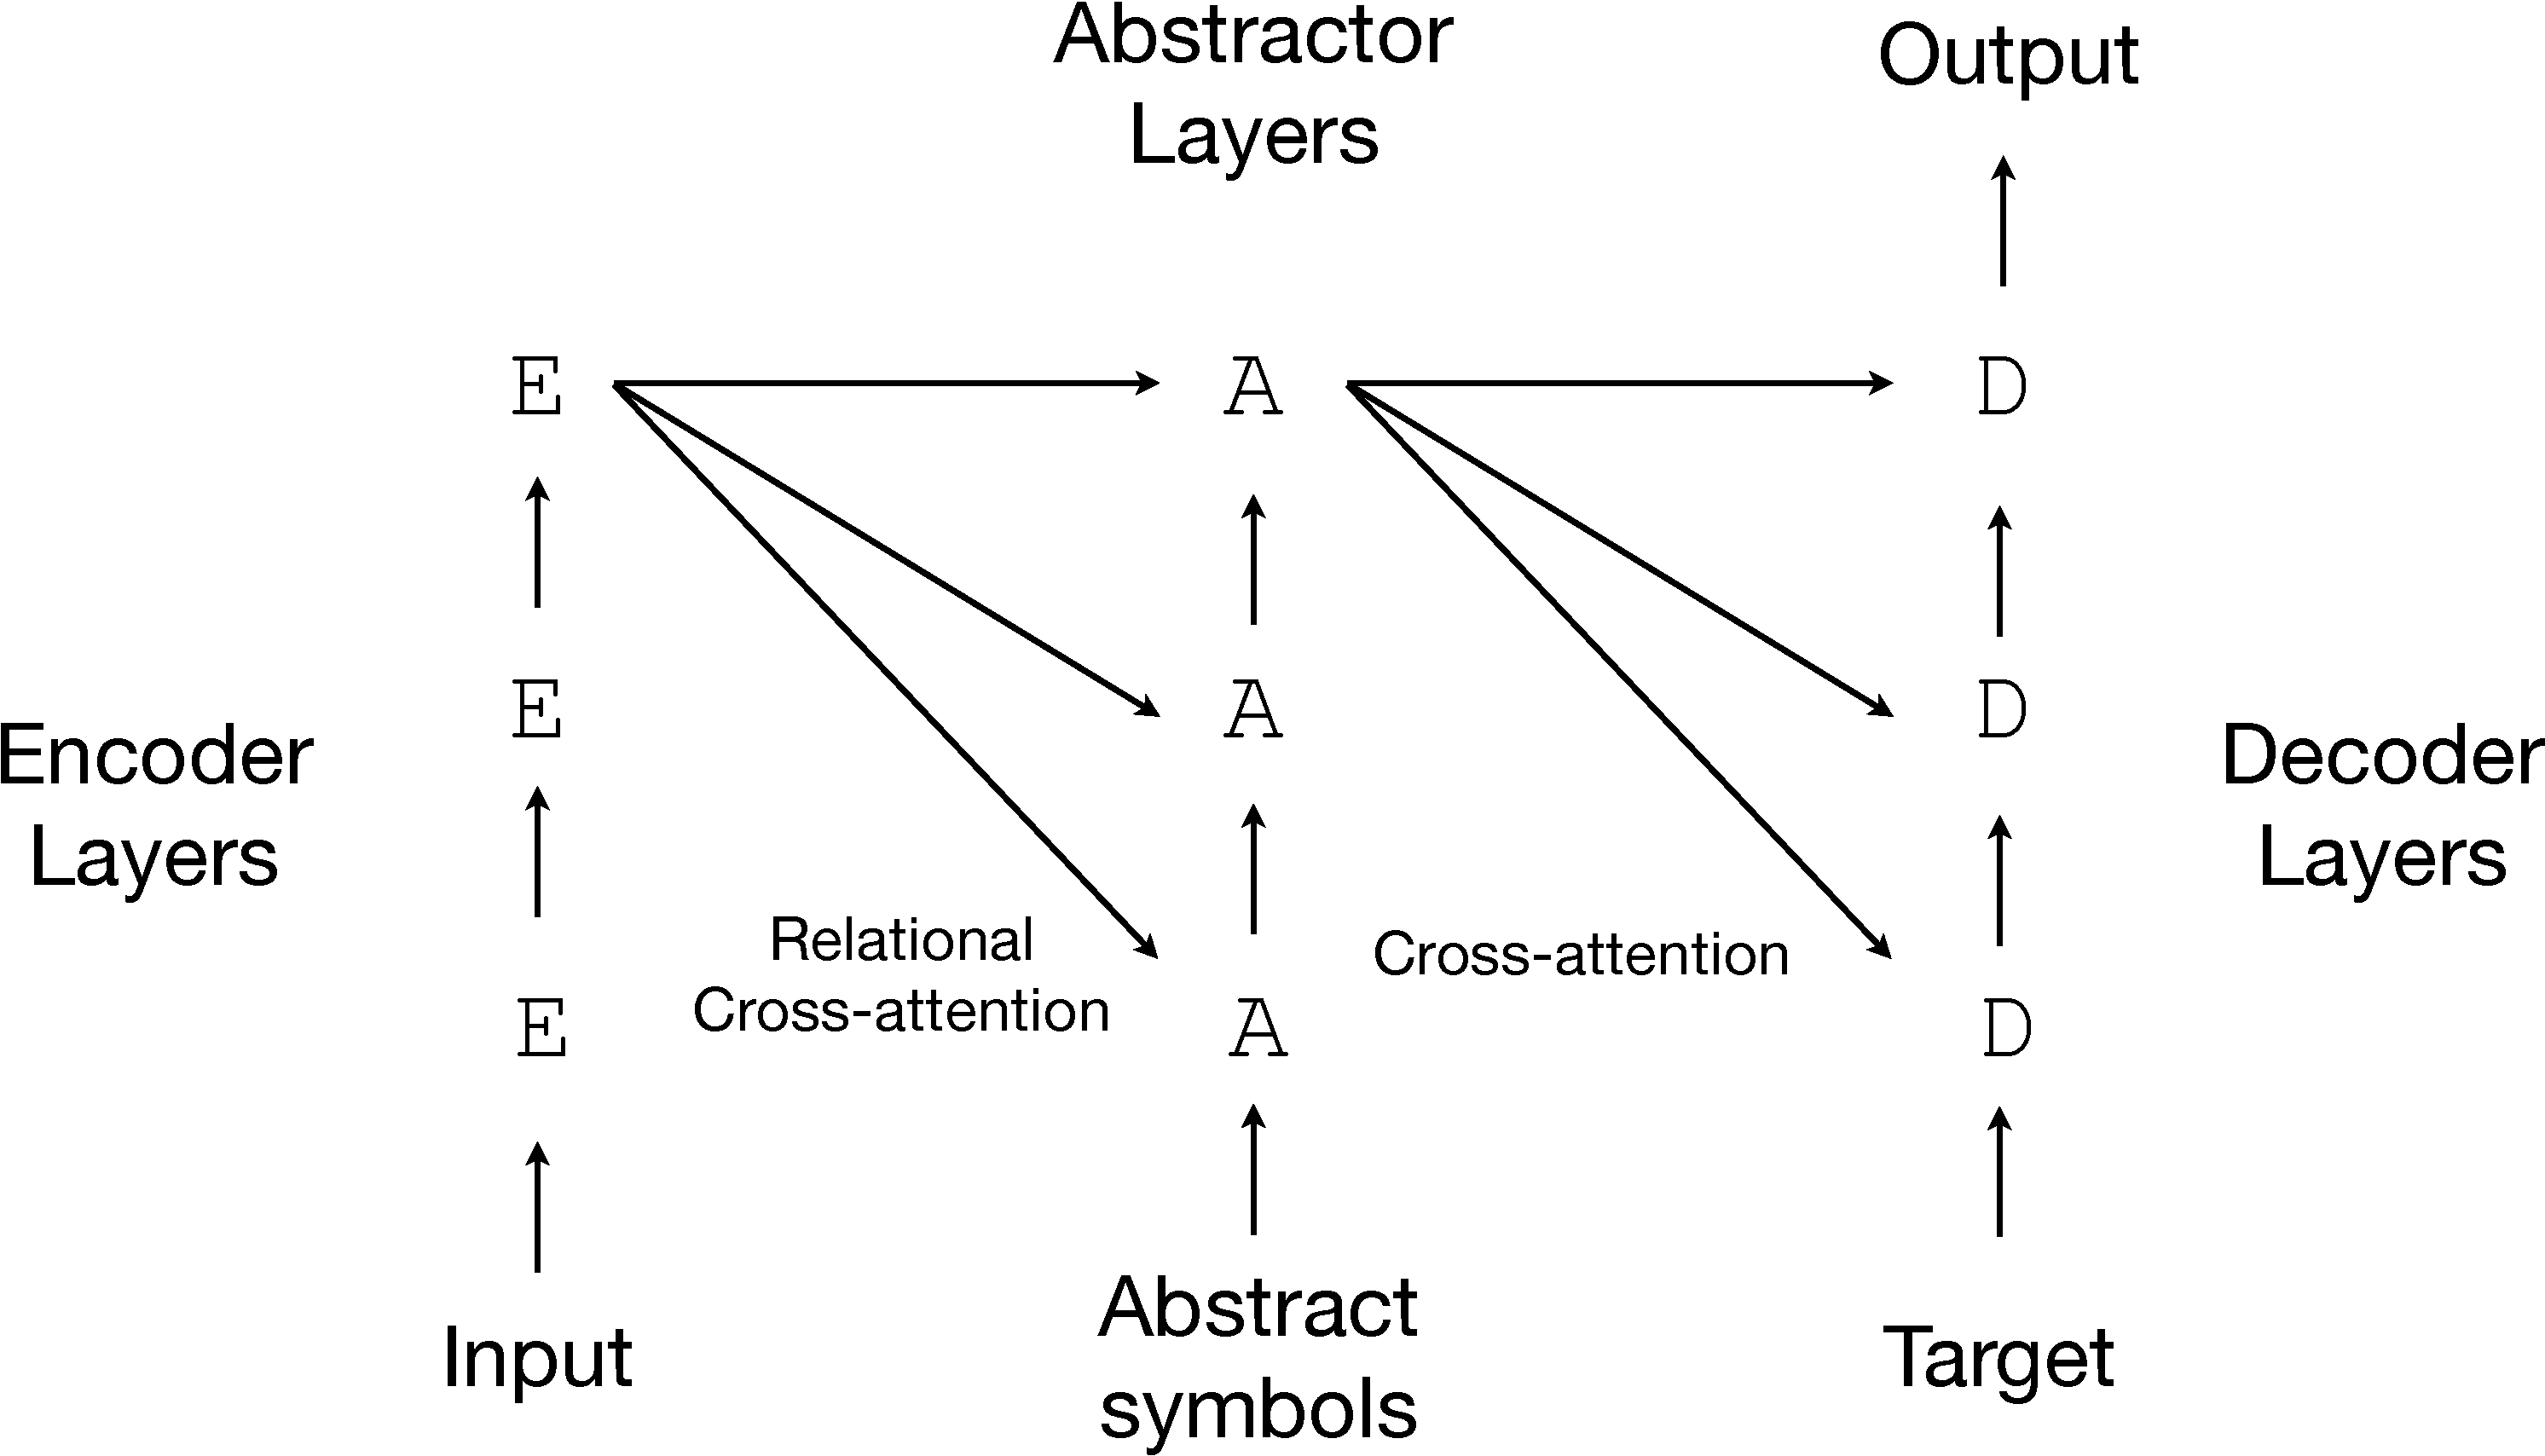
\includegraphics[width=.45\textwidth]{figures/algorithm-diagram3-crop}
        \end{tabular}
        \caption{\footnotesize Algorithmic framework integrating Transformers and relational learning, 
        implementing a form of the ``relational bottleneck.''}
        \label{fig:algo}
        \end{center}
        \vskip-.15in
    \end{wrapfigure}
    %\end{figure}
The architecture has three types of states: encoder states $E$, decoder states $D$, and abstract states $A$. The encoder states are vectors that represent domain-specific information (e.g., sensory or motor), which are often successfully modeled by standard deep learning frameworks, including standard Transformers. The abstract states $A$ are vectors that are learned and processed using symbolic message-passing based on the relations between the encoder states. In particular, the encoder states are separated from the abstract states by a ``relational bottleneck'' that only allows information about relations (that is, inner-products) between encoder states to influence the learning and transformation of abstract states.

This ability to integrate with Transformers and process domain-specific information modeled by an Encoder gives the Abstractor framework greater flexibility compared to existing relational models like ESBN.
%If sensory information is required by the decoder, this can be passed to the decoder states $D$ by standard cross-attention mechanisms of Transformers.


%
%\subsection{Example}
%\label{ssec:set}
%
%We use the game SET to illustrate relational cross-attention.
%% JDC: COULD REFERENCE WIKIPEDIA PAGE FOR SET:  https://en.wikipedia.org/wiki/Set_(card_game)
%SET is a relatively straightforward but challenging cognitive task that engages reasoning faculties in a deliberative
%, attentionally directed manner, requiring several levels of abstraction over sensory embeddings. Players are
%presented with 12 cards, each of which contains figures that vary along four dimensions (color, number, pattern, and
%shape; see Figure \ref{fig_set}a) and they must find subsets of three cards which obey a deceptively simple rule: along each dimension, all cards in a set must either have the same or unique values (e.g., in Figure \ref{fig_set}, cards with two solid blue/purple diamonds, two striped blue squiggles, and two open blue oblongs: same color, same number, different patterns, different shapes).
%
%Algorithmically, task performance can be described as follows. The visual arrangement of cards is processed into a set of encoder states $E$ by standard deep learning mechanisms. The Abstractor, starting in some initial abstract state $A$, transforms the state by the evaluation of attention heads that extract relations between the cards, each head giving a relation between them in a learned attribute.
%
%\def\redcard{\colorbox{red!30}{R}\hskip.2em}
%\def\bluecard{\colorbox{blue!30}{B}\hskip.2em}
%\def\greencard{\colorbox{green!50}{G}\hskip.2em}
%\def\onecard{\fbox{\hskip1pt 1\hskip1pt}\hskip.2em}
%\def\twocard{\fbox{\hskip1pt 2\hskip1pt}\hskip.2em}
%\def\threecard{\fbox{\hskip1pt 3\hskip1pt}\hskip.2em}
%
%\begin{figure}[t]
%\begin{center}
%\begin{tabular}{ccc}
%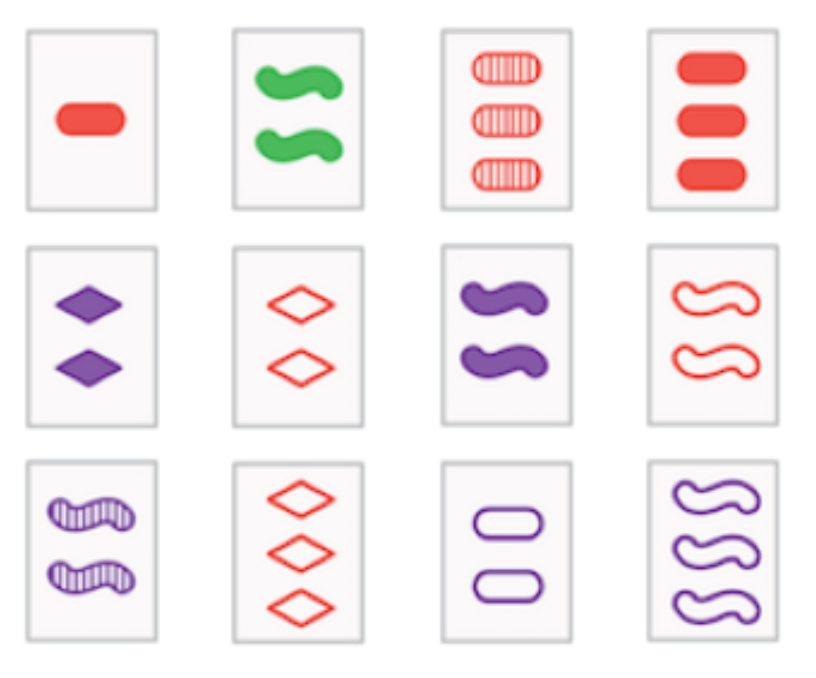
\includegraphics[width=.23\textwidth]{figures/set_example}
%& &\\[-1.15in]
%&\hskip10pt\ &\renewcommand{\arraystretch}{1.4}
%\begin{small}
%\begin{tabular}{|c|c|c|}
%%\hline
%\multicolumn{3}{c}{Attributes of encoder state $E$} \\
%\hline
%\multicolumn{1}{|c}{\redcard \redcard \redcard} & \multicolumn{1}{|c}{ \redcard\bluecard\greencard} &\multicolumn{1}{|c|}{\redcard\redcard\bluecard} \\
%\hline
%\hline
%%$\frac{1}{3}(s_1+s_2+s_3)$ & $\frac{1}{2}(s_2+s_3)$ & $s_3$ \\
%%$\frac{1}{3}(s_1+s_2+s_3)$ & $\frac{1}{2}(s_1+s_3)$ & $s_3$ \\
%%$\frac{1}{3}(s_1+s_2+s_3)$ & $\frac{1}{2}(s_1+s_2)$ & $\frac{1}{2}(s_1+s_2)$ \\
%$\frac{1}{3}(s_1+s_2+s_3)$ & $s_1$ & $\frac{1}{2}(s_1+s_2)$ \\
%$\frac{1}{3}(s_1+s_2+s_3)$ & $s_2$ & $\frac{1}{2}(s_1+s_2)$ \\
%$\frac{1}{3}(s_1+s_2+s_3)$ & $s_3$ & $s_3$ \\
%\hline
%\multicolumn{3}{c}{Transformed abstract symbol $A$}
%%\hline
%\end{tabular}
%\end{small}
%%& \\[-1.45in]
%%&&\includegraphics[width=.23\textwidth]{ppo-results/epoch_14_decision_boundaries} \vspace{-2mm} \\
%\\[10pt]
%\scriptsize (a) SET game && \scriptsize (b) Example of symbols/attention
%\end{tabular}
%\vspace{-1mm}
%\end{center}
%\caption{Illustration of mechanism used in Abstractor layers with relational cross attention using the game of SET (see text for description).
%%To provide a basic working of example of abstraction in our framework,
%As an example, consider an initial abstract symbol $S = (s_1,s_2,s_3)$ for three cards, and the color attribute.
%%, for concreteness.
%Suppose a relation is learned such that  $\langle W_Q E_i, W_K E_j\rangle$ is small if cards $i$ and $j$ have different color, and is large if they are the same color.  Then relational cross-attention transforms the initial abstract symbol $S$ as shown in the above table. A multilayer perceptron can learn to discriminate between these three cases. Once learned, the symbol $A$ then can be used to represent abstract ``same/different'' relations for the sequence of inputs.}
%\label{fig_set}
%\end{figure}
%


\subsection{Configuring Abstractors for different tasks}
\def\module#1{\mbox{\small\texttt{#1}}}

Abstractors can be used to approach a variety of relational learning tasks. In the case of classification
or regression, the default architecture would be
$$\module{Encoder} \rightarrow \module{Abstractor}$$
and the discriminant or regression function is computed as $f(A)$, where $A$ is the final abstract states.
For relational sequence-to-sequence tasks, the default architecture is
$$\module{Encoder} \rightarrow \module{Abstractor} \rightarrow \module{Decoder}$$

In a ``fully relational'' task, the decoder only attends to the Abstractor, and therefore only uses relational information from the input. Fully relational tasks are those which can be solved using only relational information, without any information about the individual objects. An example of a fully relational task is sorting objects; we give experimental details for this example in Section~\ref{sec:experiments}.

In a ``partially-relational'' task, the relational information is crucial, but information about individual objects is also important. Here, we propose an architecture in which the decoder attends to both the Abstractor and encoder modules. This can be done by either concatenating the encoder and Abstractor states (i.e.: attend to $\text{concat}(E, A)$) or to iteratively cross-attend to the Encoder and Abstractor. We call this a ``sensory-connected'' Abstractor.

% JDC: IT MIGHT BE GOOD, IF POSSIBLE TO INCLUDE AN "INLINE SCHEMATIC" FOR THIS CASE AS WELL, WITH A "BYPASS" ARROW
% (RESNET STYLE) FROM ENCODER TO DECODER (THOUGH I DON'T KNOW HOW TO DO THIS IN TEX!), TO MAKE IT VISIBLY CLEAR THAT
% THE FRAMEWORK IS FLEXIBLE.
This provides an extension of general sequence-to-sequence models with Transformers. In this paper, to highlight the capabilities of the framework, we focus our experiments on fully relational Abstractors. However, partially relational Abstractors are likely to be necessary for more realistic tasks. We hypothesize that a sensory-connected Abstractor model would yield benefits on language tasks.

We note that learning higher order relations is made possible by composing
abstractors, as in the architecture
\begin{equation*}\module{Encoder} \rightarrow \module{Abstractor} \rightarrow \module{Abstractor} \rightarrow \module{Decoder}.
\end{equation*}
Since a one-layer Abstractor is able to compute a large class of functions on relations, chaining together Abstractors allows the computation of relations on relations (higher-order relations). We formalize these comments in Section~\ref{sec:function_spaces}.

